\begin{savequote}[5cm]
The flames are silent,\\
Peace is violent,\\
Tears are frozen\\
’cause massacre was chosen.
\qauthor{--- Ankita Singhal}
\end{savequote}


\chapter[Introduction: How Terrorism Is Changing Us]{Introduction \\How Terrorism is Changing Us}
\chaptermark{Introduction}
\label{chap:chap1}

\vspace{-5mm}
\lettrine[loversize=-0.2,lines=1]{D}{}ecember 2016, on a cold, clear, winter night in the city of Brussels, I went for a drink with a group of friends. Their names were Yasser, Mohammed—who we used to call Hamudi—and Michiel. Yasser and Hamudi, both from Iraq, had arrived in Brussels just a few months earlier. They only spoke a few words of Dutch, French and English, and I only spoke a few words of Arabic. Nevertheless, through a theater play we were acting in together, we found our own way to communicate, to talk, to laugh. On that beautiful winter night in 2016, after a long rehearsal, we were having a drink, when the bartender approached us and asked me, and only me (in Dutch):

\begin{itemize}[noitemsep]
    \item[--] ``How long do you intend to stay here?''
    \item[--] ``Dunno. Why?''
    \item[--] ``We always move the tables around 8pm to start a party.''
    \item[--] ``Okay, great, then we just stay to party.'' 
    \item[--] ``Uhm, no \dots''
    \item[--] ``What, no?''
    \item[--] ``Well, \textit{you} can stay, but I prefer that \textit{they} go.''
    \item[--] ``Uhm, why?''
    \item[--] ``Well, this is Brussels and \dots you know how \textit{they} are?!''
\end{itemize}
\newpage

December 2016---the year of the terrorist attacks in Brussels and nearly one year after the Paris massacres. And so, this incident did not only infuriate me, but it also painfully reminded me of the question I was studying day in, day out: How does terrorism affect citizens' social and political attitudes?


%---------------------------------
\section{General Introduction}
\label{sec:11}
%---------------------------------

Are citizens more likely to vote for authoritarian or populist politicians in times of terror? Are they willing to compromise certain civil liberties and democratic values for greater safety and security in the wake of an attack? Do they really rally around their nation's flag, support sending troops to far-away countries, or blame Muslims and immigrants at home---like Yasser and Hamudi---for what happened? These questions are of utmost importance in today's world as various countries are currently struggling to safeguard both the safety of their citizens and some core democratic principles. Indeed, terrorism does not only shake the rule of law,\footnote{The September 11, 2001 attacks on New York City's Twin Towers and The Pentagon in Washington D.C. are well-known to have ushered in a new generation of invasive counter-terrorism policies in the United States \citep{Brooks2013, Kundnani2014}, and various European governments have taken similar measures prioritizing security, often at the expense of civil liberties, after 9/11 and other so-called terrorist attacks on European soil \citep{Bigo2015,EU2005}. This is a point I briefly return to in the conclusion, yet this dissertation predominantly concerns the drivers of \textit{popular support} for such---and other---policies.} but also the foundation of representative democracies and their legitimacy, namely the citizens \citep{VanHauwaert2020a}.


Terrorism, unlike criminal violence, is presumed at pursuing a political goal \citep{Hoffman2017, Richards2014}. It is seen by many scholars as a strategy of ``costly signaling'' or a ``weapon of the weak.'' Terrorism, according to this line of thought, is aimed at achieving political concessions by altering beliefs among a target audience because terrorists are often too weak to enforce their goals through more conventional means \citep[including traditional warfare;][p. 50]{Kydd2006}. Consequently, scholars, policymakers, and the public alike often assume that terrorism is effective to the extent it is able to affect the electorate \citep{Crenshaw1986}. Or, in other words, ``the success of this strategy relies on key assumptions about how terrorism will impact public opinion in the target state and, in turn, how these civilian responses will affect government policy towards terrorists'' \citep[][p. 1]{Wayne2019}. As a result, an impressive body of literature has accumulated---especially since the 9/11 attacks---on citizens' political responses to terrorism (see, e.g., Sniderman et al., \citeyear{Sniderman2019a} for a recent review).

%\citep[e.g.,][see also Sniderman et al., \citeyear{Sniderman2019a} for a recent review]{Brooks2013, Davis2004, Gadarian2010c, Huddy2011, Legewie2013, Merolla2009a, Vasilopoulos2019c, Vergani2018}. 


So far, this topic has been predominantly approached from a social- and political-psychological perspective (as evidenced by the preponderance of references to psychological journals in this dissertation). Collectively, these studies emphasize the role of both cognition and emotion in motivating various coping mechanisms in times of terror. Terrorism, it is hypothesized, primes the inevitability and unpredictability of death \citep{Pyszczynski2003}, prompts particular blame attributions \citep{Kimhi2009a, Sadler2005}, and triggers perceptions of risk to oneself and one's country \citep{Huddy2002a, Jost2003} as well as perceptions of injustice and moral violations \citep{Lambert2019, Skitka2002}. Terrorism also activates a complex state of negative emotional arousal. In the immediate aftermath of attacks, people feel scared and anxious, angry and outraged, sad and dejected \citep{Halperin2014, Pliskin2020}. This intertwined set of cognitions and emotions is thought to affect how citizens ``interact with the political world'' in ways that potentially put ``democracy at risk'' \citep{Merolla2009a}. Specifically, feelings of anger and moral outrage in the wake of an `unfair' attack are believed to stoke a desire for confrontational and retaliatory measures such as military action \citep{Fisk2019a, Wayne2018} or far-right voting \citep{Vasilopoulos2019c}; with fear being a major engine behind support for more preventive and precautionary measures such as the deportation of immigrants \citep{Skitka2006}, increased isolationism \citep{Huddy2005}, or counter-terrorism ethnic profiling \citep{Schildkraut2009}. 


While this research line has contributed greatly to our understanding of why and how the public responds to terrorism, the core argument of this dissertation is to widen its \textit{conceptual}, \textit{theoretical}, and \textit{empirical} scope. In particular, I argue that, while cognitive and affective mechanisms remain an excellent starting point to understand why and how terrorism affects citizens, solely relying on social- and political-psychological studies risks painting an inaccurate and incomplete picture due to three main gaps. First, conceptually, despite a burgeoning literature on the relationship between `terrorism' and sociopolitical attitudes, there is \textbf{insufficient engagement with the conceptualization of `terrorism'} within this particular field of study. As Chapter 5 demonstrates, the vast majority of the empirical studies on public reactions to terrorism refrains from clearly and explicitly defining terrorism and, hence, makes the unfounded---although often implicit---assumption that `terrorism' is a clear-cut `you-know-it-when-you-see-it' phenomenon. However, as we will discover throughout this dissertation, the way citizens think and talk about `terrorism' forms an integral part of how this concept is changing them and the particular societies they live in. Hence, this dissertation calls for a more conscious and critical engagement with the core concept, `terrorism,' and shows how an intergroup perspective offers a useful framework for our understanding of both the conceptualization of and responses to `terrorism.'


Second, theoretically, several strands of literature (especially within psychology, political science, and media studies) have approached the topic of this dissertation from different angles, but there is \textbf{no real dialogue yet between these different paradigms.} This is an important gap as different disciplines tend to focus on different levels of analysis. For example, most studies in the field of social- and political-psychology have focused on the unique role of individual-level cognitions and emotions within single-case studies \citep[e.g.,][]{Huddy2005,Canetti-Nisim2009b, Vasilopoulos2019c}. As a result, much less is known about the contextual factors that foster or impede the impact of such cognitions and emotions on opinion formation in times of terror. Both media studies and political science research, by contrast, often employ comparative research designs to assess more structural, macro-level determinants (such as the role of power dynamics or elite cues and discourses). To date, only a handful of studies integrate these individual and aggregate levels of analysis \citep[e.g.,][]{Legewie2013, Nussio2019, Castanhosilva2018}.


Third, empirically, studies examining how the public reacts to terrorism are still \textbf{predominantly conducted within Western settings}, especially within the United States \citep[see, e.g., the prominent books of][]{Albertson2015, Davis2007, Merolla2009a,Pyszczynski2003} and Europe \citep[e.g.,][]{Legewie2013, Nussio2019, Castanhosilva2018}, \textbf{or Israel} \citep[e.g.,][see also Chapter 5 for an empirical proof of this argument]{Kalagy2017, Canetti2009, Halperin2009b, Hall2009, Feinstein2018}. This Western/Israeli focus raises important questions about the generalizability of commonly used theories in the field today. Indeed, one of the central observations of this dissertation is that the effects of acts of violence depend on the political and societal context in which they occur. Societies, in turn, are characterized by their own history, norms, socio-demographic realities, discourses, power relations, and more. All of this influences the way citizens perceive ‘terrorism’ in the first place, and how this may change their social and political attitudes. Yet, our knowledge of how terrorism changes citizens and societies across different, and especially within non-Western, societies remains very limited. 


Overall, despite the ever-growing interest in and importance of understanding public reactions to terrorism, some crucial questions remain unanswered. More specifically, much of the existing literature is still characterized by an uncritical engagement with the concept of `terrorism,' a narrow focus on micro-level determinants, and a Western/Israeli-centered geographical scope. Consequently, the central aim of this thesis is to advance knowledge on how terrorism influences citizens' attitudes by asking the following overarching research questions: \textit{(1) How does terrorism affect citizens' social and political attitudes? And (2) how can we explain differences in attitudinal reactions between individuals and across societies?}


To comprehensively answer these questions, the next section begins by laying out the overarching conceptual and theoretical framework. This framework primarily draws on insights from social and political psychology, and integrates these insights with theory and research originating from political sciences and media studies. More specifically, it extends earlier work on the psychological drivers of public reactions to terrorism by, first, engaging critically with the concept that lies at the heart of this relationship (i.e., ‘terrorism’) and, second, grounding it in a more rigorous and context-sensitive theoretical foundation. Such integrative and interdisciplinary conceptual and theoretical framework,\footnote{As the framework ``analyzes, synthesizes and harmonizes links between disciplines into a coordinated and coherent whole,'' it falls under the category ``interdisciplinary'' \citep[][p. 351]{Choi2006}.} I argue, holds greater explanatory power because it identifies and tests the importance of constructs, originating from different disciplines, at both the individual and contextual level. In the empirical chapters, this framework is then put to the test by employing a cross-national comparative approach (Chapters 2 and 5) and an in-depth case-study of the Boko Haram conflict in Nigeria (Chapters 3 and 4). The former approach is used to examine the influence of several contextual factors, whereas the latter contributes to assessing how `terrorism' is changing citizens in non-Western societies. In this respect, the Boko Haram conflict in Nigeria is considered a particularly useful and highly instructive case-study. 


First, Nigeria constitutes one of the countries that have suffered most from terrorism, yet are barely studied. Indeed, although Afghanistan, Iraq, \textit{Nigeria}, Syria, and Pakistan remain the five countries most affected by terrorism \citep{TheInstituteForEconomicsAndPeace2019}, we still know surprisingly little about how people in these countries cope with such severe and sustained threat because most research tends to focus on the impact of singular transnational attacks within Western settings or sustained violence in Israel. When it comes to Boko Haram, this homegrown insurgency has killed tens of thousands and displaced millions of people since the escalation of violence in 2009 \citep{Campbell2019}. In 2014, this Jihadist movement was even denounced the world's deadliest terror group \citep{InstituteforEconomics&Peace2015}. Moreover, Boko Haram has its origins in the northeastern city Maiduguri and primarily operates in the North-East of Nigeria and the wider region around Lake Chad. Its root causes can be traced back to a dynamic combination of Nigeria's turbulent history and particularly its post-1999 politics, poverty and relative deprivation, youth bulges and agency, geographical factors, and religious doctrines \citep{Mustapha2014b, Thurston2018, Onuoha2010, Onuoha2012}. More information on the history and root causes of Boko Haram can be found in Appendix \ref{app:A1}.


Second, the Boko Haram conflict also constitutes an interesting case-study given Nigeria's intergroup context. More specifically, Christians and Muslims each constitute about half of the Nigerian population \citep{NPC2013} and, since independence, individuals from both religious groups have held powerful positions \citep[such as those of military ruler and president;][]{Mustapha2009, Nnoli1996}. This is in sharp contrast to the often-studied Western and Israeli societies, where Muslims are usually a small and relatively marginalized minority. This is an important remark given that, to this day, the relationship between terrorism and attitudes has almost exclusively been studied from the perspective of a clear-cut majority in-group in the context of Islamist, and thus out-group, violence (see Chapter 5). In other words, most previous work has been conducted in a context where the in- and out-group boundaries and dynamics are clear. Yet, the implications of this intergroup reality are rarely acknowledged---let alone addressed in-depth. I aim to fill this gap by systematically studying how Islamist violence (i.e., Boko Haram violence) has affected sociopolitical attitudes in a starkly different and less delineated intergroup context (i.e., Nigeria).


This deeper focus on a non-Western context (Chapter 3 and 4) as well as the broader focus across societies (Chapter 2) and this field of study as such (Chapter 5), has inspired the main argument of this dissertation. More specifically, in the conclusion, I will argue that it might not be terrorism as such that is changing citizens, but rather the \textit{`idea} of terrorism'---an idea determined to a large extent by \textit{specificities of the intergroup context} in which threats or acts of violence take place. Throughout this dissertation, the Nigerian case-study will bring to light the potentially crucial role played by, first, the delineation of the fault lines and corresponding groups within a conflict and, second, consequent micro-level contact and macro-level power hierarchies between those groups. Such specificities of the intergroup context contribute to this idea of terrorism and, thereby, to mitigating (or aggravating) terrorism-induced attitudinal effects (Chapter 6). %Therefore, the framework outlined in the next Section, including the conceptualization of the \textit{`idea} of terrorism,' will be further extended in the conclusion based on the empirical chapters by putting it into an {intergroup perspective}. 


In sum, this dissertation aims to contribute to the literature by combining a critical and intergroup perspective on the concept of `terrorism' with psychological predictions of its effects and by empirically testing these predictions across national contexts and methodological paradigms. In the remainder of this chapter, I outline the interdisciplinary conceptual and theoretical framework guiding this dissertation (Section \ref{sec:12}) and present a brief overview of the specific research questions, methodological approaches, and data sources upon which the empirical chapters build (Section \ref{sec:13}). While the former section further clarifies the conceptual and theoretical contributions of this dissertation, the latter highlights its empirical and methodological innovations.


%------------------------------------------------
\newpage
\section{Conceptual and Theoretical Framework}
\label{sec:12}
%------------------------------------------------

In this dissertation, I advance a novel interdisciplinary and integrative framework to contribute to current understandings of how `terrorism' is changing citizens and societies. The framework contains, first, a comprehensive and critical engagement with the definition of terrorism and, second, an integration of several theoretical perspectives explaining why and how terrorism affects public attitudes. To do so, I build upon different traditions of research which, so far, have been developed in comparative isolation. More specifically, I borrow key insights from theories originating from \textit{social and political psychology} (such as, terror management theory, motivated social-cognition approach, appraisal theories, and affective intelligence theory), \textit{media studies} (such as, agenda-setting, priming, and framing theories, exemplification theory, and the spiral of silence), and \textit{political sciences} (such as, rally-around-the-flag, issue ownership theory, and social-constructivist perspectives like securitization theory). Table \ref{tab:intro-app-tab1} in Appendix \ref{app:A2} briefly summarizes the main theories used and their corresponding disciplines, while Figure \ref{fig:intro-app-fig1} provides a glimpse of the mind-mapping technique used to structure all theories into one single framework. It is worth noting that this framework originated gradually based on crucial insights gained throughout the doctoral project. Consequently, individual pieces of it will reappear in the empirical chapters, and the concluding chapter will add a final argument to this framework based on the collection of empirical findings.


At its core, the conceptual and theoretical framework guiding this dissertation builds upon four arguments. First, `terrorism' should be conceptualized as a multifaceted, context-depending phenomenon comprising particular acts or threats of violence coupled with the words, images, and counteracts used by political elites and mass media. In other words, in this dissertation, I see both acts or threats of violence and elite's labelling of those acts/threats as terrorism as necessary elements for something to be terrorism. Collectively, I label this the `idea of terrorism.' Second, this idea triggers an intertwined set of unconscious and conscious, cognitive and affective reactions. Third, this complex cognitive and affective state, in turn, may affect citizens' attitudes towards other people, politicians, policies, and politics in general. As we will see, it often causes citizens to bolster their attachment to the in-group, while simultaneously derogate those that do not belong to this critical inner circle. Last, citizens' reactions to `terrorism' are not uniform but often conditioned by both dispositional and contextual factors, including characteristics of the `idea of terrorism,' of the societies in which citizens live and their own predispositions, and of the specific attitudes susceptible to change. 


In short, a complex combination of cognitive and affective, dispositional and contextual factors is thought to shape citizens' sociopolitical reactions to `terrorism.' Although such reactions might be short-lived \citep{Sniderman2019a}, they may still hold long-lasting implications by feeding reactionary policies \citep{Tomz2019} and the narratives of extremist organizations \citep{Bail2018}.\footnote{Unfortunately, empirically testing feedback loops falls outside the scope of this dissertation.} Figure \ref{fig:intro-theory} visualizes the broad interconnections between the main elements of the overarching framework, whereas the four central arguments are further developed in the next sections based on existing literature. 



%----------------------------------------------------------
% Figure 1: Theoretical framework
%----------------------------------------------------------
\begin{figure}[H]
\centering
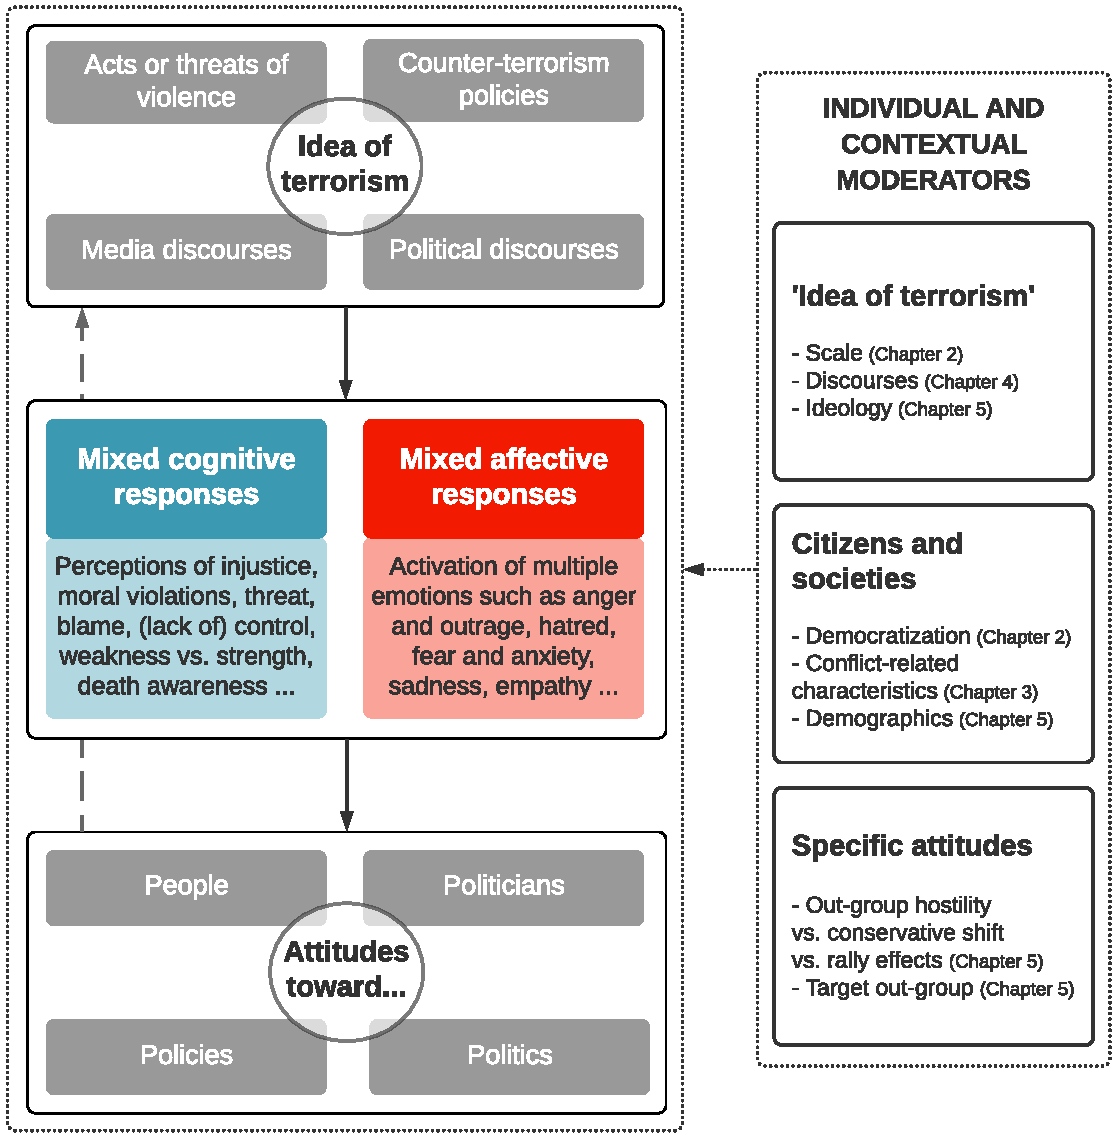
\includegraphics[width=0.96\textwidth]{Chapter_1/intro-figure1.pdf}
\caption{Conceptual and Theoretical Framework}
\label{fig:intro-theory}    
\end{figure}
\newpage
%----------------------------------------------------------



%----------------------------------------------------------
\subsection{Argument 1: The `Idea of Terrorism'}
\label{sec:121}
%----------------------------------------------------------
Just like nearly every article or book written on this topic, I start by embracing the compulsory line acknowledging that terrorism is, first and foremost, a highly contentious and contested concept.\footnote{Interestingly, in my meta-analysis (Chapter 5), I actually found that, while this is true for studies originating from (critical) terrorism studies, it does not hold for those empirical studies looking at public attitudes changes after so-called terrorist attacks. In fact, only a handful of the +200 studies included in my meta-analysis explicitly stated how they defined `terrorism.'} This contention is probably best summarized in the cliché statement ``one man's terrorist is another man's freedom fighter\textit{.}'' Throughout this dissertation, and as a result of this conceptual blur and contestation, I actually follow three definitional approaches---which might seem confusing at first. However, as a dissertation project entails a learning trajectory, my understanding of terrorism as a concept developed throughout the empirical studies I conducted. These different conceptualizations thus reflect my instructive academic journey and feed into the first argument concerning the `idea of terrorism.' Here follows a snapshot of my academic adventure diary.


In Chapter 2, I embark upon this academic journey by following the \textbf{academic consensus definition of terrorism} \citep{Schmid2011} and operationalizing it using the Global Terrorism Index \citep{TheInstituteforEconomicsandPeace2016}. In the academic literature, terrorism is often defined as (1) \textit{violence,} or at least the threat\footnote{Including the threat of violence is more common among scholarly definitions compared to policy definitions. One of the possible reasons for this disparity is the difficulty to detect and, consequently, deter threats of violence. Yet, although threat is a vague aspect hard to---legally---pin down, it is an extremely useful concept within political psychology and, hence, for this dissertation. For a lengthy discussion of the role of threat in defining `terrorism', see \cite{Brown2020}. For some of the first accounts of the influential role of threat in activating political intolerance, see \cite{Stouffer1955} or Sullivan and colleagues (\citeyear{Sullivan1981, Sullivan1982}).} of violence, (2) aimed at evoking a \textit{psychological effect,} (3) in order to achieve a \textit{political goal }\citep[e.g.,][]{Richards2014}. Some definitions go beyond this to further delimit the scope of terrorism and specify characteristics of the victims, perpetrators, and/or tactics. What marks acts of violence as terrorism, according to this line of thought, is the deliberate targeting of \textit{civilians or non-combatants }\citep[e.g.,][]{Schmid2011} by \textit{non-state or subnational actors }\citep[e.g.,][this criterion is also used in the Global Terrorism Index]{LaFree2015}.\footnote{This non-state actors criterion is quite interesting if you consider that many scholars locate the origins of the term in Maximilien Robespierre’s Reign of Terror (1793-1794) during the French Revolution. See Erlenbusch (\citeyear{Erlenbusch2015}) for a critical perspective on the emergence of `terrorism' in the French Revolution.} And, in part because of this noncombatant target or non-state perpetrator, some have argued that one of the distinctive features of terrorism is its clear ``\textit{violation of established norms}''  \citep[][p. 3]{Laqueur1987}. 


Feeling slightly uncomfortable with this conventional approach (but not yet realizing why), I took a step back from defining the term by studying\textbf{ specific actors and their usage of the tactics and vocabulary of terrorism and counter-terrorism.} While Chapter 3 examines the determinants of Nigerians' willingness to reintegrate ex-Boko Haram fighters, Chapter 4 reveals how Boko Haram has been covered in two Nigerian newspapers. The crucial role played by the media in times of conflict, including terrorism, has long been recognized and studied by political and communication scientists alike \citep[e.g.,][]{Wolfsfeld2004, Tenenboim-Weinblatt2016}. In fact, terrorism is quite unique in this respect since it is often explicitly conceptualized as a communication strategy where ``the immediate human victims [...] serve as message generators [...] used to manipulate the main target'' \citep[][p. 28]{Schmid1988}.


The way terrorism is portrayed in the media is therefore crucial to understand why people respond to terrorism in certain ways. In this regard, Shanto Iyengar (\citeyear{Iyengar1991}) found that terrorism news receives a disproportionate amount of coverage and is predominantly framed in a so-called episodic way, excluding any historical, economic, or social context.\footnote{This finding is consistent with many other content analyses of conflict news coverage \citep[][p. 152]{Tenenboim-Weinblatt2016}, including the one in Chapter 4 in this dissertation.} Founding father of framing studies, Robert Entman (\citeyear{Entman2003}), further showed how the Bush administration's `war on terror' frame of the 9/11 attacks provides ``a textbook example of high magnitude, high resonance framing'' by putting all blame on the terrorists, condemning them as ``evil wrongdoers,'' and propagating a war against these evil perpetrators as the only effective remedy (p. 417). This `war of terror' frame was barely challenged by democratic leaders and, as a result, overwhelmingly dominated the news in the direct aftermath of the attacks \citep{Entman2003, Glazier2012}.\footnote{This stifling of elite dissent engenders what Elizabeth \cite{NoelleNeumann1974} has called `a spiral of silence.' The `spiral of silence' notion has parallels with the Brody-Shapiro (\citeyear{Brody1989}) model of opinion leadership. Brody and Shapiro (\citeyear{Brody1989}) argue that, at their onset, international crises ``usually (but do not always) substantially alter the normal partisan character of the information available to the public. (\dots) opposition political leaders either tend to refrain from critical comment or to make cautiously supportive statements'' (p. 355).} Furthermore, scholars have also documented a double standard, in which mass media (and political institutions alike) are more likely to apply the `terrorist' label and adopt a generic `Islamic terror frame' when the perpetrator of an attack is (or is perceived to be) Muslim, but are more likely to explore the perpetrators' personal life and mental health when they are not \citep{Powell2011}. In part as a result of such media and elite framing, citizens equally tend to label acts of violence more often as terrorism when they are carried out by Muslims \citep{DOrazio2018, Huff2018} and form their political opinions accordingly \citep{Piazza2015}. Collectively, these studies thus outline a critical role for media and political discourses in answering the question of how terrorism is changing us \citep[see also][]{Nacos2011, Terrorism}. Accordingly, any inquiry into the relationship between terrorism and socio-political attitudes should not only consider particular acts of violence, but also how elites talk about such violence.


Building on this line of thought, in the final two chapters, I came to understand and study `terrorism' as \textbf{a multi-faceted and complex social and political phenomenon}. It comprises specific forms of acts and/or threats of violence coupled with the words, images, and actions of politicians and journalists (with the `war on terror' probably the most dominant frame and counter-act advocated in the twenty-first century). Notably, all of this is always embedded within and determined by a given social and political context. David Rapoport's (\citeyear{Rapoport2004}) well-known wave theory highlights the importance of taking context, in particular history, into account. He defines a terrorist wave as ``a cycle of activity in a given time period---a cycle characterized by expansion and contraction phases'' \citep[][p. 47]{Rapoport2004}, and identifies four waves of modern terrorism: the Anarchist Wave (1880s-1920s), Anti-Colonial Wave (1920s--1960s), New Left Wave (1960s--1980s), and Religious Wave (1990s to Present). Similarly, Jessica Stern (\citeyear{Stern2003}) has referred to terrorism as a ``Protean Enemy,'' underlining its constantly changing nature. And Lisa Stampnitzky (\citeyear{Stampnitzky2013}, 141) compellingly argues that ``the Soviet Union has been cast as an existential threat to `the West' throughout the 1980s,'' with Islam being the ``new number one national enemy'' nowadays. 


Critical terrorism scholars, like Stampnitzky, often draw on social-constructivist ideas in general \citep{Wendt1992} and securitization theory in particular \citep{Buzan1998, Buzan1983} to explain this constantly changing nature of the ``Protean Enemy.'' Securitization theory describes how elites within a given society at a particular moment in time try to securitize various phenomena, including ideologies and religion, by using ``\textit{performative }speech acts.'' Elites securitize these phenomena by not just declaring them as threatening but as an ``existential security threat'' \citep[][p. 171--172; original emphasis]{Jorgensen2010}. Such existential threats, in turn, create what Agamben (\citeyear{Agamben2005}) calls a ``state of exception,'' necessitating and justifying an extraordinary policy response (such as the war on terror).\footnote{The parallel with the field of media studies is noteworthy. Yet, this fields often calls these performative speech acts ``frames'' and draws more regularly on hegemonic theory \citep{Gramsci2009}, instead of securitization theory, to explain the dominance of certain frames within a society. Entman (\citeyear{Entman2003}), for example, applies hegemonic theory to explain framing in the context of 9/11. However, see also Meier's (\citeyear{Meier2019}) theory of hegemonic components of national identity within International Relations. } 


To reiterate, I conceptualize `terrorism' as a context-depending phenomenon comprising certain acts or threats of violence assumed to pursue a political goal, coupled with the words, images, and acts of mass media and political elites. I thus include within the conceptualization of terrorism a variety of (a) forms of violence, (b) policy responses, and (c) political and (d) media narratives (which includes demarcating labels, attributed causes, and propagated solutions). Taken together, I label this the `idea of terrorism.' Importantly, in the conclusion, I add one final element to this conceptualization by further illustrating how this \textit{`idea'} is embedded within and influenced by a given sociopolitical, and particularly intergroup, context (see Section \ref{sec:611}). Yet first, in what follows, I explore the main mechanisms underlying public reactions to this `idea of terrorism.'\footnote{In the remainder of this thesis, I will use the terms `terrorism,' `terror,' and the `idea of terrorism' interchangeably. Please remember that `terrorism/terror' always refers to this complex interplay of both acts and discourses of terrorism and counter-terrorism.}


%----------------------------------------------------------
\subsection{Argument 2: A Complex Set of Mediators }
\label{sec:122}
%----------------------------------------------------------
For nearly a century, social scientists have attempted to understand why instances and periods of threat affect citizens' political and social ideas, attitudes, and behaviors. As a result, various theoretical perspectives have emerged to explain the political aftermath of threat in general and terrorism in particular.  These theories share two general assumptions. First, they emphasize that ``all threats involve the experience of discrepancy'' \citep[][p. 221]{Jonas2014}. Indeed, Festinger's (\citeyear{Festinger1975}) cognitive dissonance theory (CDT) forms a central element across the social and political psychological literature, including extant theories on threat.\footnote{CDT holds that people have a strong desire for cognitive consistency. As a result, any discrepant experience that conflicts with prevailing cognitions will cause aversive arousal and motivate people to adjust their thoughts and behaviors to reduce this arousal \citep{Jonas2014}. Cognitive dissonance may be induced by both individual acts (e.g., engaging in counter-attitudinal behavior such as smoking while knowing its dangers) and situational contexts (e.g., instances and periods of violence; Jonas et al. 2014).} Second, to cope with existential and collective threats, such as terrorism, most theories expect people to use coping mechanisms that transcend individual actions. Specifically, shifts in ``attitudes, evaluations, and behaviors with respect to other individuals, policies leaders, and other nation states'' are often-hypothesized collective coping mechanisms in times of terrorism \citep[][p. 10]{Merolla2009a}. Yet, while aversive arousal and collective coping underlie most theories on threat/terrorism and public attitudes, there are noteworthy differences between existing theories as to the centrality of cognitions versus emotions in inciting this arousal. 


On a \textbf{cognitive} level, terrorism is thought to prime the unpredictability and inevitability of death \citep{Pyszczynski2003}, prompt particular blame attributions \citep{Kimhi2009a, Sadler2005}, trigger the idea that oneself and one’s country is in danger \citep{Huddy2002, Jost2003}, and heighten perceptions of injustice and moral violations \citep{Lambert2019, Skitka2002}. At a more abstract level, terrorism thus challenges basic human assumptions about the world as being predictable, safe, and benign (Cannetti et al. \citeyear{Canetti2013a}, p. 267; see also shattered assumptions theory by Janoff-Bulman, \citeyear{Janoff-Bulman1992}). The \textit{motivated social cognition} framework argues that, when confronted with ``a world that appears dangerous and unpredictable,'' people---even self-identified liberals---will adhere more strongly to ``conservative, authoritarian, and right-wing candidates, policies, and ideologies'' \citep[][pp. 326-327]{Jost2017a}. A set of interrelated epistemic and existential motives to manage uncertainty and threat underlie this so-called conservative shift \citep{Jost2003, Jost2017a}. Several empirical studies corroborate with this conservative-shift hypothesis by revealing increases in support for more intrusive surveillance measures \citep[e.g.,][]{Davis2004}, military intervention \citep[e.g.,][]{Gadarian2010c, Fisk2019a}, anti-immigration policies \citep[e.g.,][]{Ferwerda2017}, and far-right parties and politicians \citep[e.g.,][]{Vasilopoulos2019c} in times of terrorism.


%By contrast, \textit{terror management theory}---the second main theory within this field of study---states that, under life-threatening circumstances, people will strengthen their own worldviews (including ideological predispositions), which may lead to political polarization instead of conservatism \citep{Pyszczynski2003}. 


On an \textbf{affective} level, terrorism is thought to elicit many forms of negative affect, including fear, anger, and sadness. One of the major advances in political psychology of the last decade, is the increased emphasis on specific or so-called `discrete' emotions. While the dominant approach has long been to identify the unique roles played by positive versus negative affect in explaining human behavior, recent studies have demonstrated how discrete emotions of the same valence may entail different effects in the context of intergroup conflict \citep{Pliskin2020}. In the realm of terrorism studies, scholars have predominantly focused on the impact of fear and anger. In this respect, fearful individuals are shown to support more risk-aversive, defensive, and preventive actions \citep{Huddy2005, Lerner2003a, Skitka2006}, with feelings of anger and moral outrage being major drivers of support for more high-risk, punitive, and retributive actions \citep{Fisk2019a, Skitka2006, Wayne2018}.\footnote{The relative impact of fear and anger is hotly debated today, with some scholars arguing that attitudinal responses in times of terror are ``more likely built upon the public’s anger rather than fear'' \citep[][p. 267]{Vasilopoulos2019c} and others stating that anger mediates the effect of fear on political responses \citep{Jost2019}. See the whole exchange between Vasilopoulos et al. and Jost in Political Psychology (2019) for more information.} 
%Sadness, although far less studied than anger and fear, is shown to prompt empathetic and altruistic behavior \citep{Conejero2007}.


It is, however, important to note that ``in the post-Freudian world, the ancient dichotomy between reason and passion is blurred'' \citep[][p. 340]{Jost2003}. In other words, I follow Sniderman and colleagues (\citeyear{Sniderman2019a}) by seeing attitudinal responses in times of terror as ``jointly dependent on automatic, affective responses and supervisory cognitive functions. Consistent with a standard dual-processing model, emotional responses automatically activated by a terror attacks, with some effort, can be subject to conscious control'' (p. 255). Such conscious or cognitive reasoning, in turn, may again feed emotions \citep{Moors2013}. Indeed, appraisal theories conceive emotions as ``adaptive responses which reflect appraisals of features of the environment that are significant for the organism’s well-being'' \citep[][p. 119]{Moors2013}. In sum, terrorism is related to conscious and unconscious cognitions and emotions which are intertwined in a complex and circular way. This web of mediators is thought to underlie attitudinal responses to terrorism and, in what follows, I look at the concrete configuration of these responses.

 
%----------------------------------------------------------
\subsection{Argument 3: A Complex Set of Attitudinal Responses}
\label{sec:123}
%----------------------------------------------------------
The third argument central to the theoretical framework guiding this dissertation holds that a complex state of cognitive and affective reactions to the `idea of terrorism' leads to\textbf{ several shifts in social and political attitudes}. In times of collective crises, citizens tend to look for solutions beyond their individual actions, and changes in one's sociopolitical attitudes and beliefs are deemed effective collective coping mechanisms in this regard \citep{Merolla2009a}. In this dissertation, both political and social attitudes are bundled in what I call the `4Ps' of attitudinal responses in times of terror. More specifically, attitudes related to particular people, politicians, policies, and politics in general are thought to shift, at least temporarily, in times of terror. Table \ref{tab:intro-tab1} displays some examples of these four clusters of attitudes, whereas the next paragraphs further outline some of the exact consequences of terrorism for these `4Ps.'


\vspace{3mm}
%----------------------------------------
% Table 1
%----------------------------------------
%\begin{table}[H]
%\caption{The `4Ps' of Attitudinal Responses in Times of Terror}
%\label{tab:intro-tab1.1}
%\onehalfspacing
%\begin{tabular}{@{}p{3.3cm}|p{2.8cm}|p{3.3cm}|p{3.3cm}@{}}
%\toprule
%People              & Politicians   & Policies              & Politics \\ \midrule
%Out-group hostility & Approval      & National security     & Political ideology \\
%In-group solidarity & Trust         & Military intervention & Political trust \\
%Generalized trust   & Support (vote)& Immigration policies  & Nationalism \\ \bottomrule
%\end{tabular}
%\end{table}
%----------------------------------------
% Please add the following required packages to your document preamble:
% \usepackage{booktabs}
\begingroup
\small
\onehalfspacing
\begin{longtable}[H]{@{}p{0.5cm}L{4cm}L{8.5cm}@{}}
\caption{The `4Ps' of Attitudinal Responses in Times of Terror}
\label{tab:intro-tab1}\\
\toprule
\multicolumn{2}{l}{Attitudes towards...} & Examples \\
\hline
\endfirsthead
%
\multicolumn{3}{c}%
{{Table \thetable\ continued \dots}} \\
\hline
\multicolumn{2}{l}{Attitudes towards...} & Examples \\ \hline
\endhead
\hline
\multicolumn{3}{r}{\textit{Continued on next page}} \\
\endfoot
\hline
\endlastfoot
%
\multicolumn{2}{l}{... People} &  \\
 & Generalized trust & \cite{Geys2017, Clark2013a, Wollebk2012} \\
 & Out-group hostility & \cite{Echebarria-Echabe2006, Legewie2013, Ferwerda2017, Ciftci2012, Panagopoulos2006}\\
 & In-group solidarity & \cite{VanHauwaert2020a} \\
\multicolumn{2}{l}{... Politicians} &  \\
 & Evaluations & \cite{Holman2017, Merolla2007, Ladd2007, Lambert2010, Merolla2009a, Merolla2009b} \\
 & Electoral support &  \cite{Aytac2019a, Gilboa1990a, Bali2007, Montalvo2011, Berrebi2008a}\\
\multicolumn{2}{l}{... Policies} &  \\
 & National security & \cite{Davis2004, Davis2007, Brinson2012b, Blauwkamp2018, Gadarian2010c, Bali2009, Baele2019} \\
 & Military retaliation & \cite{Bar-Tal2001, Fisk2019a, Gadarian2010c, Gross2017, Rovenpor2019, Feinstein2018, Canetti2017, Grizzard2017}  \\
 & Immigration policies & \cite{Kim2016, Ferwerda2017, Boomgaarden2006a, Canetti2009, Castanhosilva2018, Finseraas2013c, Canetti-Nisim2008a} \\
\multicolumn{2}{l}{... Politics in general} &  \\
 & Political ideology &  \cite{Vasilopoulos2018, Asbrock2013a, Bonanno2006, Barnes2012, Canetti2017}\\
 & Political trust and civic/vote engagement & \cite{Larsen2020, Robbins2013, Koch2016, Eshel2016a, Kimhi2019, Arvanitidis2016}  \\
 & Nationalism and patriotism &  \cite{Barnes2012, Henderson-King2009, Lambert2010, Feinstein2018}\\
 \bottomrule
\end{longtable}
\endgroup

On the one hand, terrorism is thought to enhance national sentiments, political trust, and support for national leaders \citep[e.g.,][]{Moskalenko2006, Dinesen2013a, Feinstein2018, Landau2004, Ladd2007, Lambert2010}. This is often collectively labelled as a `rally-around-the-flag' effect. In 1973, Meuller defined a rally event as ``(1) international, (2) involving the US and especially the President, and (3) specific, dramatic, and sharply focused'' (p. 209). Such rally events were initially hypothesized to cause a surge in presidential approval by increasing patriotism and elite consensus \citep{Brody1989, Baker2001, Berinsky2009, Mueller1970, Mueller1973}, but the theory was latter applied to equally explain upsurges in different forms of institutional trust inside and outside the US in times of different crises.\footnote{Merolla and colleagues show, however, how not every leader gets an equal boost in popularity after rally events. Across different studies (related to terrorism), they point to the relative gains bestowed on politicians to the extent that they are male, incumbents, running on the Republican ticket, and perceived as charismatic and strong leaders experienced in national security affairs \citep{Holman2019a, Holman2011, Holman2016a, Merolla2007, Merolla2009a, Merolla2009b, Merolla2013}.} 


On the other hand, terrorism is hypothesized to increase intolerance towards out-groups in general \citep[e.g.,][]{Echebarria-Echabe2006} and Muslims, Arabs, and immigrants/refugees in particular \citep[e.g.,][]{Panagopoulos2006, Argyrides2004, Ciftci2012, Hopkins2010a, Ferwerda2017}. Indeed, one of the most consistent findings in social psychology is the power of threat ``to increase intolerance, prejudice, ethnocentrism, and xenophobia, regardless of whether threat is defined as a widely acknowledged external force or a subjective, perceived state” \citep[][p. 594]{Huddy2005}. This often translates into support for restrictions on the rights and liberties of those disliked groups \citep[e.g.,][]{Davis2007} or stricter anti-immigration policies \citep[e.g.,][]{Kim2016}.\footnote{However, see more nuanced results in \cite{Legewie2013} or \cite{Nussio2019} and null results in \cite{Castanhosilva2018} or \cite{Larsen2020}.} Not only policy choices regarding out-groups are affected in times of terror, but evidence also points in the direction of a general desire for retribution---especially among those who feel angry because of terrorism \citep{Wayne2018}. For example, studies have documented an increased support for retaliatory, military, and conflict-perpetuating---instead of conciliatory and diplomatic---solutions to conflict \citep{Bar-Tal2001, Rovenpor2019}, a stronger preference for national security at the expense of civil liberties \citep{Davis2004}, and a greater tendency to vote for far-right parties and politicians \citep{Vasilopoulos2019c}. These responses are often collectively seen as evidence for a shift towards the conservative end of the political spectrum in times of threat. Yet, the `conservative shift' hypothesis goes one step further by also predicting attitudinal changes across a wider range of policy issues and deep-seated political beliefs \citep[such as one's general ideological leaning;][see also Section \ref{sec:122}]{Jost2003, Jost2017a}.\footnote{In a similar vein, the issue ownership literature suggests that certain political parties and ideologies in general will benefit when `their' issue becomes more salient \citep{Petrocik1996, Seeberg2017}. As right-wing parties are considered to be associated with addressing security threats, they are thought to benefit when security concerns increase \citep{GETMANSKY2014, Aytac2019a}.} 


Both \textit{social identity theory} \citep[SIT;][]{Tajfel1979} and the \textit{coalitional index model} \citep{Boyer2015} help to explain these particular dynamics in public responses to terrorism. It is commonly acknowledged that people are intrinsically motivated to achieve or maintain a ``positive social identity,'' and that this identity is largely based ``on favorable comparisons that can be made between the in-group and some relevant out-groups'' \citep[][p. 40]{Tajfel1979}.\footnote{In 1979, Tajfel and Turner aptly named the collection of these ideas the “social-identity social-comparison theory” (p. 41), yet the label “social identity theory” became more widely used.} Evolutionary psychology adds that the tendency to perceive the world in terms of in-groups and out-groups is based on the fact that intergroup conflict has been substantial enough to constitute a selection pressure \citep{Tooby2010}. In other words, intergroup relations have been and still are ``strongly influenced by threat-detection mechanisms'' \citep[][p. 435]{Boyer2015}. Being part of a group is psychologically comforting and any threat to that equanimity needs to be carefully managed. The detection of threats---both real or imagined---therefore results in coping attitudes and behaviours ranging from bolstering in-group alliances and commitments to avoiding or competing against out-group members and alliances \citep{Boyer2015, Lindner2018}. While these ideas pertain to threat in general, SIT and coalitional psychology are particularly powerful theories in the context of the threat of terrorism as they illustrate how the empirical evidence outlined above maps onto such processes of in-group solidarity and out-group hostility. Specifically, while rally effects are often targeted at in-group members, attitudes studied in the conservative shift literature regularly pertain to out-groups.\footnote{One might rightly wonder why I draw on SIT and coalition psychology instead of on another prominent theory within the study of terrorism effects: \textit{terror management theory }\citep[TMT;][]{Pyszczynski2003, Rosenblatt1989, Greenberg1986}. TMT equally posits that threat may stimulate in-group favoritism and out-group derogation or, in TMT terminology, `worldview defenses.' However, \textit{death-related cognitions} are central to activating such defenses within TMT, whereas SIT and coalition psychology suggest that it might not be death-related cognitions as such but rather existential \textit{out-group} threats that might be driving reactions. In other words, SIT and coalition psychology also help us to explain why certain threats or acts of violence are more likely to be perceived as terrorism and, hence, elicit public reactions. Specifically, terrorism is something `they' inflict on `us.' This argument is further developed in the conclusion (Chapter 6) based on existing theoretical notions and the empirical findings of this dissertation. }



%----------------------------------------------------------
\newpage
\subsection{Argument 4: A Complex Set of Moderators}
\label{sec:124}
%----------------------------------------------------------
The final argument of the theoretical model states that such attitudinal responses to terrorism are not uniform. Instead, both \textbf{micro- and macro-level moderators} are thought to influence whether or not, how, and to what extent `terrorism' affects attitudes. More specifically, characteristics of the citizens themselves, the societies in which they live, and the terrorist threats under scrutiny are thought to moderate public reactions to terrorism.


First, various studies have documented the impact of individual-level moderators, including standard demographics such as gender and ethnicity as well as more specific moderators such the inclination to affiliate with the in-group and motivation to control prejudice. While results regarding ethnicity and the corresponding status of someone's ethnic group are mixed and context-dependent \citep{Shoshani2016, Lavi2014}, men are generally more likely to endorse harsh and hawkish counter-terrorism policies \citep{Huddy2005, Lindner2018a, Lizotte2017}. In addition, given that attitudinal reactions to terrorism are a collective or group-level coping strategy, people who identify more strongly with the in-group are also thought to react more strongly to terrorism (Asbrock \& Fritsche, \citeyear{Asbrock2013a}; but see null results in Bilali, \citeyear{Bilali2015}). On the other hand, studies have also documented factors inhibiting the development of hostile attitudes in response to terrorism such as a higher internal motivation to control prejudice \citep{Steen-Johnsen2019, Sobolewska2017} or one's level of political knowledge \citep{Carriere2019a}.


When it comes to individual-level moderators, a particularly contested and so far unresolved question is whether and how political predispositions shape public reactions to terrorism remains. Whereas the reactive-liberal hypothesis \citep{Nail2009a} argues that liberals will be more inclined to toward reactive conservatism as a defense mechanism against threat, terror management theory \citep{Pyszczynski2003} suggests that death-related thoughts and concerns will stimulate citizens to embrace their own worldviews and pre-existing beliefs---causing liberals to become more liberal and conservatives to become more conservative. Empirically, Van de Vyver et al. (2016) and Hetherington and Suhay (2011) found evidence for the reactive-liberal hypothesis and Castano et al. (\citeyear{Castano2011}) for the worldview defense hypothesis, for example. Yet, Castanho Silva (\citeyear{Castanhosilva2018}) found neither an overall shift in immigration attitudes nor significant differences in attitudes between liberals and conservatives in response to the series of attacks in France in 2015. In sum, both existing theoretical predictions and empirical findings regarding the moderating role of political predispositions are mixed.


Second, a handful of studies have also unravelled the effect of country- or context-level moderators, such as unemployment rates \citep{Legewie2013, Castanhosilva2018}, the local migration context \citep{Nussio2019, Legewie2013}, and geographical proximity to particular attacks \citep{Nussio2019}. Collectively, these studies support the notion that contextual vulnerability---indicated by higher unemployment and lower education rates \citep{Legewie2013, Castanhosilva2018} but not by geographical proximity to terrorist attacks \citep{Nussio2019}---leads to stronger out-group hostility reactions in the wake of terrorism. In addition, the local migration context has been hypothesized to matter. As local populations have less experience with immigration in more homogeneous societies, views immigrants and refugees are thought to be more strongly affected in those relatively homogeneous contexts \citep{Nussio2019}. 


Last, in addition to individual- and country- or context-specific moderators, citizens are also found to be more supportive of extraordinary measures against male terror suspects compared to their female counterparts \citep{Lindner2018a} and against suspects identified as Muslims compared to their right-wing counterparts \citep{Piazza2015}. The specific way in which news outlets construe terrorist threats and acts also influences how citizens will respond to them. Previous studies suggest, for example, that framing collective trauma in inclusive rather than exclusive terms (i.e., `we are all in this together,' see Canetti et al. \citeyear{Canetti2018a}) or explicitly distinguishing between the perpetrators of the violence and the larger group to which they belong (i.e., `Jihadi terrorists are not Muslims,' see von Sikorski et al. \citeyear{VonSikorski2017}) can mitigate detrimental effects of violence, whereas emotionally powerful visuals might aggravate these detrimental effects \citep{Gadarian2010c}. 



This dissertation adds a few important moderators to this non-exhaustive list. In Chapter 2, we draw on notions of community resilience to hypothesize that the association between terror and trust is moderated by a country's \textit{political and media environment}. In Chapter 3, building on political psychology, we expect heterogeneous treatment effects to our conjoint experiment depending on respondents' \textit{conflict-related characteristics}. And Chapter 5 uses meta-regression techniques to assess the impact of a wide range \textit{research design features} on the strength of the relationship between terrorism and sociopolitical attitudes. Last, while these hypotheses are tested in a primarily deductive fashion, the conclusion in Chapter 6 adds a final moderator in an inductive and theory-building way. Here, based on the empirical findings of this dissertation, I illustrate the crucial, but often overlooked, implications of the \textit{intergroup context} in which acts and threats of political violence take place. To avoid abundant repetition, I refer to the respective chapters for the theoretical elaboration of the predictions for each moderator.



%----------------------------------------------------------
\newpage
\section{Plan of this Dissertation}
\label{sec:13}
%----------------------------------------------------------
This dissertation consists of a collection of four empirical articles. Collectively, the articles contribute to answering the overarching research questions (as asked in Section \ref{sec:11}) and fit into the conceptual and theoretical framework (as proposed in Section \ref{sec:12}). As this is an article-based dissertation, some parts of this overarching framework will reappear in the theory section of the individual chapters. Each article is also guided by its own specific research gaps and questions which, in turn, has informed the respective empirical approaches used. Consequently, each article employs a different data collection method, operationalization of key variables, and analytical approach---which allows for a robust test of the relationship between terrorism and public attitudes across settings, methods, and indicators. Yet, in developing these empirical approaches, there were three general guiding principles: applying cross-national designs, focusing on a non-western case-study, and unravelling moderators and mediators. Furthermore, as one will see, the articles are ordered chronologically (meaning by the time I initiated them over the course of my doctoral project). As a result, particular questions raised by the results of one article directly feed into the research questions and designs of the next article. In what follows, I shortly outline the aim and scope of all articles (which I will call chapters from now on) and highlight how they engage with the overarching research questions and goals as discussed above. Table \ref{tab:intro-tab3} at the end of this chapter presents an overview of the specific research questions, data sources, and analytical approaches per chapter.


\textbf{Chapter 2}, entitled \textit{'Does Terror(ism) Destroy Trust?'}, responds to the dearth of comparative research within the field of terrorism effects studies, by focusing on the complex relationship between terrorism and trust across different societies worldwide. Although social trust is often referred to as `the glue that binds societies together,' our understanding of whether and how `terrorism' affects this `glue' remains fairly limited. To fill this academic void, we combine individual-level data of the most recent World Values Survey (2010-2014; N\textsubscript{individuals} = 76,254; N\textsubscript{countries} = 54) with country-level indicators (in particular the Global Terrorism Index). Applying multi-level modeling, we examine the relationship between a country's objective terrorist threat level, citizens' perceptions of this threat, and the extent to which they trust people in general. The findings clearly show that terrorism (i.e., particular acts of violence) and terror (i.e., the psychological effect of such violence) are two separate phenomena, in which the latter is particularly harmful to our social fabric. Next, we ask what drives this `terror of terrorism' and show that, first, objective threat still has an indirect effect on trust by increasing citizens' threat perceptions and, second, that television news consumption equally catalyzes such threat perceptions. Finally, we hypothesize and confirm that the relationship between terror and trust is not uniform across countries, but moderated by a country's level of democratization and---albeit to a weaker extent---objective danger. The article, therefore, ends with an intriguing puzzle: Why is the relationship between fear of terrorism and social trust \textit{non-existent} in less democratic, and more terrorist-prone, countries? This puzzle serves as a fundamental building block for the subsequent articles and the selection of Nigeria as the case-study on which this dissertation draws.


\textbf{Chapter 3}, entitled \textit{'How to Forgive Former Fighters?'}, zooms in on one specific policy-attitude. Particularly, by employing a conjoint experiment, we aim to unravel some of the preconditions and circumstances under which Nigerian young adults (N = 1,930) would be more likely to support the reintegration of former members of violent extremist groups. Although community acceptance of reintegration is often recognized as a \textit{sine qua non} for reintegration to be successful, it is rarely addressed in-depth. This Chapter, therefore, introduces a typology of reintegration attitudes. Building on peace research and conflict resolution literature, we first examine the causal impact of seven features of ex-fighters on Nigerians' willingness to reintegrate them. These attributes are related to characteristics of the individual ex-fighters themselves, the atrocities they have committed, and the actions they have undertaken since leaving the insurgency. The results show a greater willingness to reintegrate those ex-fighters that show signs of remorse, repentance, and reconciliation. Respondents’ belief in the success of post-conflict reintegration seems to be an important mechanism driving these attitudes. Second, drawing on political psychology, we also analyze the moderating power of conflict-related civilian characteristics (operationalized via the religious background of our respondents as well as their encounters with and anger toward Boko Haram violence). Do Nigerians hold different reintegration preferences depending on their religious background, conflict exposure, or anger responses? In sharp contrast to prior studies, we find no evidence for any of the hypothesized moderators. And hence, Chapter 3 equally ends with an intriguing puzzle: Why do Christians and Muslims, victims and non-victims, and angry and non-angry respondents \textit{react in the same way} on our conjoint experiment?


\textbf{Chapter 4}, entitled \textit{`Hey, They Aren't Muslim!'}, provides one possible answer to the two intriguing questions that arose from Chapter 2 and Chapter 3 by taking news coverage of `terrorism' into account. In this chapter, we meticulously document Boko Haram coverage in both a Northern-based/Muslim-affiliated and a Southern-based/Christian-affiliated Nigerian newspaper, and interview Nigerian media practitioners to understand why they cover the insurgency in particular ways. Based on a quantitative content analysis of 711 news articles, we find that, while Nigerian newspapers tend to adopt a war-oriented narrative (which is in line with Western news coverage), they generally do not associate Boko Haram's violence with Islam and Muslims as such (which is in contrast to much Western news coverage). This absence of an association is found in both the Northern-based (and, hence, Muslim-affiliated) newspaper ànd the Southern-based (and, hence, Christian-affiliated) newspaper. Overall, the two newspapers reported in very similar ways on the Boko Haram crisis--—which again contradicts the often-assumed ethnocentric bias inherent in terrorism news. This chapter therefore concludes that it is crucial to pay closer attention to a country’s political-religious demography to better understand the way in which religious-based violence is covered in the news. In this respect, we identify a micro-, meso-, and macro-level theoretical mechanism through which a country’s demography can promote domestic news outlets—regardless of their background and readership—to cover conflict in a more balanced, nuanced, and objective way.


\textbf{Chapter 5}, entitled \textit{`Does Terrorism Really Affect Attitudes?'}, takes stock of the existing empirical evidence for the often-assumed relationship between terrorism and sociopolitical attitudes. To date, the field of terrorism effects studies still lacks a systematic review of the available information---one that outlines key features of this field of study, consolidates the overall effect size, and unravels potential moderators. To address these gaps, I perform a three-level meta-analysis of 1,709 effect sizes quantifying the relationship between terrorism and sociopolitical attitudes (including out-group hostility, political conservatism, and rally-around-the-flag measures). The results confirm that terrorism is associated with small increases in out-group hostility and political conservatism, but not, as often assumed, with unequivocal rally-around-the-flag effects. Here, the effects are predominantly driven by a rally-behind President Bush effect. At the same time, the review reveals important gaps and methodological issues within this body of scholarship. At its core, it illustrates how the question of how terrorism affects attitudes, in fact, boils down to the much narrower question of how \textit{Islamic} terrorism affects attitudes in \textit{Western} societies. The meta-analysis, therefore, also sheds light on important biases, assumptions, and scope conditions underlying and characterizing this field of study. %It helps to understand why I expected one-sided media reporting or polarized attitudes between Christians and Muslims in Nigeria (Chapter 3 and 4), or why I was surprised finding out that the relationship between fear and social trust disappears when citizens have most to fear (Chapter 2).

\textbf{Chapter 6}, finally, integrates these empirical findings into an overarching conclusion emphasizing the need for a more context-sensitive study of terrorism effects, discusses the limitations of this dissertation, and outlines several promising avenues for future research.

%----------------------------------------------------------
% Table 1.1. Overview of Dissertation
%----------------------------------------------------------
\begin{table}[H]
\small
\caption{Overview of Specific Research Questions, Data Sources, and Analytical Approaches Used in Each Chapter of this Dissertation} 
\label{tab:intro-tab3}
\renewcommand{\arraystretch}{1.5} %spacing between rows
\begin{tabular}{@{}cp{4cm}p{4cm}p{3.7cm}@{}}
\toprule
\multicolumn{1}{l}{Ch.} & Research Question(s) & Data Source(s) & Analytical Approach(es) \\ \midrule
2 & How far does terrorism as well as the fear of future terrorism destroy social trust among different individuals and societies across the world? & World Values Survey 6 (n\textsubscript{countries} = 54; n\textsubscript{individuals} = 76,254) merged with country-level indicators (in particular the Global Terrorism Index) & Multi-Level Models and Multi-Level Structural Equation Models \\
3 & Which factors foster or impede popular support for the reintegration of former members of violent extremist groups? & A conjoint experiment in Nigeria. Subjects
were presented pairs of ex-Boko Haram members and asked which ex-fighter they prefer to reintegrate and how successful they thought the reintegration process of the ex-fighters would be (n = 1,930) & Estimation of average marginal component effects (AMCEs) and marginal means (MMs) for main and sub-group analyses (i.e., moderation based on subjects' religion, exposure to Boko Haram violence, and anger responses)  \\
4 & How do Nigerian media report on Boko Haram, and how can we explain similarities and differences between Western and Nigerian media in terms of out-group representation of Muslims? &
\parbox[t]{3.5cm}{(1) 26 in-depth expert interviews with Nigerian journalists and editors \\ (2) A unique database of 711 Nigerian newspaper articles} & \parbox[t]{3.5cm}{(1) Systematic coding \\ (2) Exploratory quantitative content analysis} \\
5   & How strong is the evidence for the relationship between terrorism and sociopolitical attitudes and which factors aggravate or attenuate this relationship? & Meta-analytic dataset of 235 reports on this topic (which covers 317 unique samples, 1,709 effect sizes, and +400,000 respondents) &  Three-level meta-analysis and -regressions \\ \bottomrule
\end{tabular}
\vspace{-3mm}
\singlespacing
\footnotesize{\textit{Note:} The sample sizes refer to the effective sample size used in the analyses (i.e., after list-wise deletion).}\par
\end{table}
\clearpage



